\section*{Problem 2}
Repeat problem 1 for the following signal:

\begin{figure}[H]
\caption*{}
\centering
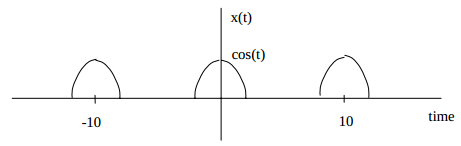
\includegraphics[width=0.8\textwidth]{figs/c1p2.png}
\label{fig:c1p2}
\end{figure} 

\subsection*{Solution}
The period of the shown signal is $T=10$ and therefore $\omega_0 = \frac{2 \pi}{T} =  \frac{\pi}{5}$.

If we take the first and second derivative of $x(t)$ we get:

\begin{figure}[H]
\caption{Derivative $\dot{x}$}
\centering
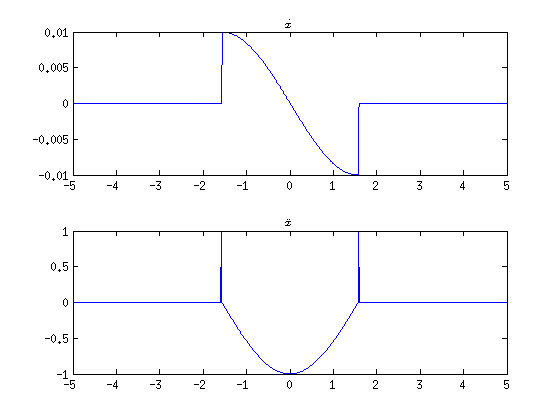
\includegraphics[width=0.8\textwidth]{figs/c1p2a.png}
\label{fig:c1p2a}
\end{figure} 

The range t = [-5,5] contains one complete period of the signal.
Applying (\ref{eq:c12}) we have:

\begin{equation*}
\begin{aligned}
\ddot{x}(t) &= - x(t) + \delta(t+\pi/2) + \delta(t-\pi/2)\\
\displaystyle\sum_{- \infty}^{\infty} - n^2 \omega_0^2 X_n e^{j n \omega_0 t} &=
\displaystyle\sum_{- \infty}^{\infty} X_n e^{j n \omega_0 t} + 
\delta(t+\pi/2) + \delta(t-\pi/2) \\
\displaystyle\sum_{- \infty}^{\infty} (1 - n^2 \omega_0^2) X_n e^{j n \omega_0 t} &=
\delta(t+\pi/2) + \delta(t-\pi/2) \\
\end{aligned}
\end{equation*} 

Whe can now obtain $X_n$ with:

\begin{equation*}
\begin{aligned}
(1 - n^2 \omega_0^2) X_n &= \frac{1}{T} \int_{-5}^5 \delta(t+\pi/2) + \delta(t-\pi/2) 
e^{-j n \omega_0 t} \; dt \\
&=\frac{1}{T} ( e^{j n \frac{\omega_0}{2}} + e^{- j n \frac{\omega_0}{2}} ) \\
X_n &= \frac{1}{5(1-\frac{n^2 \pi^2}{25})} \cos(\frac{n \pi^2}{10})
\end{aligned}
\end{equation*} 

Next we use Matlab to plot the magnitude and phase of the spectra using the script given in \cite{wprobl_c1}

\zcodemat{sources/c1p2.m}{Calculate and plot magnitude and phase of Xn}

\begin{figure}[H]
\caption{Magnitude and Angle $X_n$}
\centering
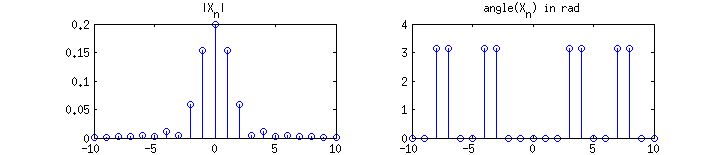
\includegraphics[width=0.8\textwidth]{figs/c1p2b.png}
\label{fig:c1p1b}
\end{figure} 

We then plot the approximation of the function using its Fourier coefficients 
\cite{wprobl_c1}.

\zcodemat{sources/fapprox2.m}{Approximation of x(t) with Fourier coefficients}

\begin{figure}[H]
\caption{Approximation of x(t) by Xn}
\centering
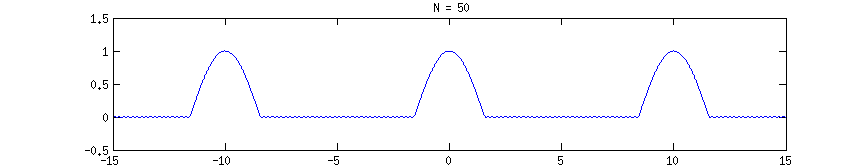
\includegraphics[width=0.8\textwidth]{figs/c1p2c.png}
\label{fig:c1p1c}
\end{figure} 
